\begin{figure}[h]
  \centering
  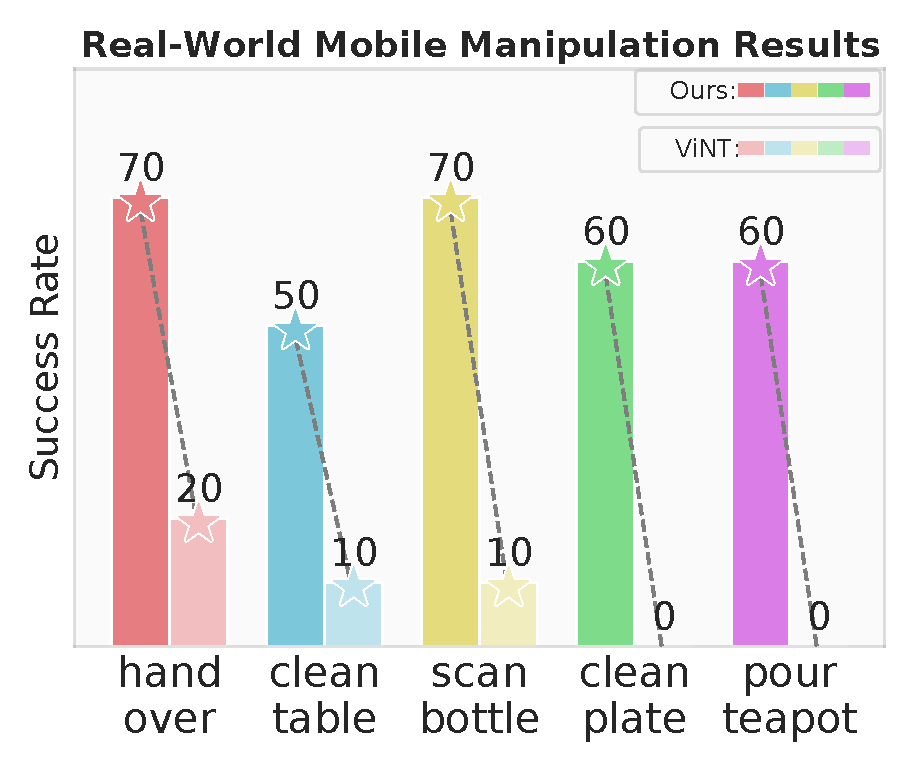
\includegraphics[width=1.0\linewidth]{figures/manipulation_bar_pic.pdf}
  \vspace{-15pt}
  \caption{ \textbf{Real-world mobile manipulation results.} Dark-colored bars correspond to \ourshort, whereas the light-colored bars correspond to only using ViNT. \ourshort is capable of performing a wide array of complex mobile bimanual dexterous manipulation tasks. In contrast, when relying solely on ViNT for localization, the trained manipulation policy fails to complete the tasks. } 
  \label{fig:mani_bar}
\end{figure}